\begin{frame}{The Engine: Resampling Strategies}
    \begin{center}
    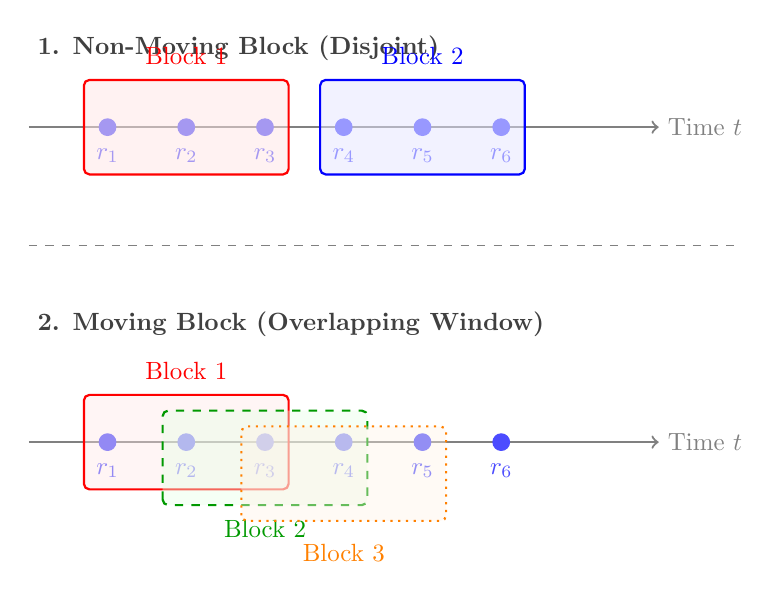
\begin{tikzpicture}[scale=1, every node/.style={scale=0.9}]

        % --- NON-MOVING BLOCK ---
        \node[anchor=west, font=\bfseries\color{darkgray}] at (0, 2) {1. Non-Moving Block (Disjoint)};
        \draw[->, thick, gray] (0, 1) -- (8, 1) node[right] {Time $t$};
        \foreach \x/\label in {1/r_1, 2/r_2, 3/r_3, 4/r_4, 5/r_5, 6/r_6} {
            \filldraw[blue!70] (\x, 1) circle (3pt) node[below=5pt] {$\label$};
        }
        % Blocks
        \draw[thick, red, rounded corners=2pt, fill=red!10, fill opacity=0.5] (0.7, 0.4) rectangle (3.3, 1.6);
        \node[text=red] at (2, 1.9) {Block 1};
        \draw[thick, blue, rounded corners=2pt
        , fill=blue!10, fill opacity=0.5] (3.7, 0.4) rectangle (6.3, 1.6);
        \node[text=blue] at (5, 1.9) {Block 2};

        \draw[dashed, gray] (0, -0.5) -- (9, -0.5); % Separator

        % --- MOVING BLOCK ---
        \node[anchor=west, font=\bfseries\color{darkgray}] at (0, -1.5) {2. Moving Block (Overlapping Window)};
        \draw[->, thick, gray] (0, -3) -- (8, -3) node[right] {Time $t$};
        \foreach \x/\label in {1/r_1, 2/r_2, 3/r_3, 4/r_4, 5/r_5, 6/r_6} {
            \filldraw[blue!70] (\x, -3) circle (3pt) node[below=5pt] {$\label$};
        }
        % Overlapping Blocks
        \draw[thick, red, rounded corners=2pt, fill=red!10, fill opacity=0.4] (0.7, -3.6) rectangle (3.3, -2.4);
        \node[text=red] at (2, -2.1) {Block 1};

        \draw[thick, green!60!black, dashed, rounded corners=2pt, fill=green!10, fill opacity=0.4] (1.7, -3.8) rectangle (4.3, -2.6);
        \node[text=green!60!black] at (3, -4.1) {Block 2};

        \draw[thick, orange, dotted, rounded corners=2pt, fill=orange!10, fill opacity=0.4] (2.7, -4.0) rectangle (5.3, -2.8);
        \node[text=orange] at (4, -4.4) {Block 3};

    \end{tikzpicture}
    \end{center}
\end{frame}